\documentclass{standalone}
\usepackage{standalone}
\usepackage{tikz}
\usepackage{graphicx}
\usepackage{float}
\usepackage{listings}
\usepackage{caption}
\usepackage{fancyhdr}
\begin{document}
% \begin{framed}
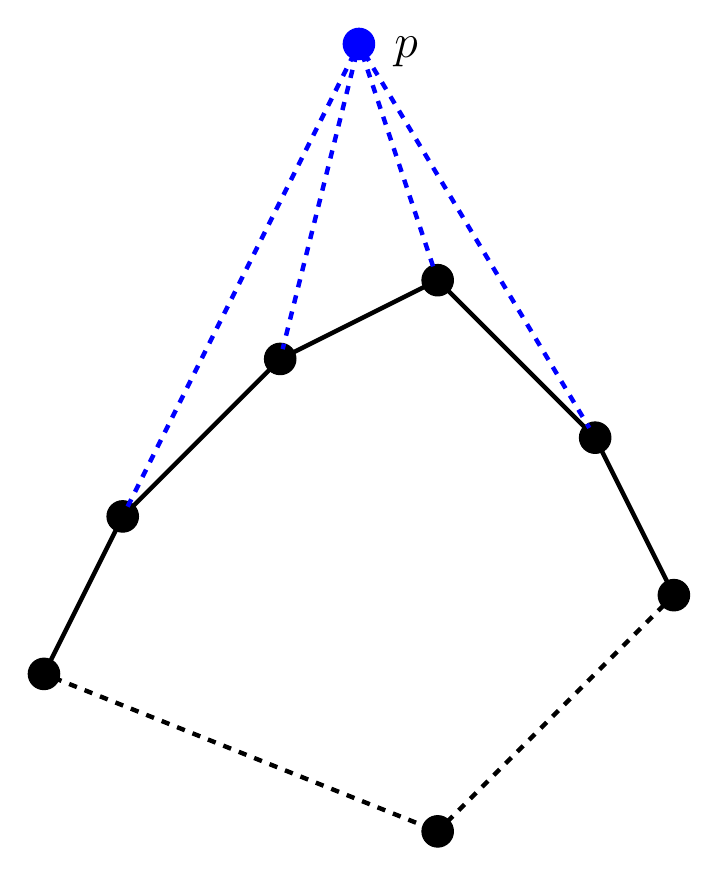
\begin{tikzpicture}
\node (a) at (0, 0) {};
\node (b) at (1, 2) {};
\node (c) at (3, 4) {};
\node (d) at (5, 5) {};
\node (e) at (7, 3) {};
\node (f) at (8, 1) {};
\node (g) at (5,-2) {};
\node (p) at (4, 8) {};

\filldraw (a) circle (.2) (b) circle (.2) (c) circle (.2) (d) circle (.2) (e) circle (.2) (f) circle (.2) (g) circle (.2) ;
\draw[ultra thick] (a)--(b) (b)--(c) (c)--(d) (d)--(e) (e)--(f);
\draw[dashed, ultra thick] (a)--(g) (f)--(g);
\filldraw[color=blue] (p) circle (.2);
\draw[dashed, ultra thick, color=blue] (p)--(b) (p)--(c) (p)--(d) (p)--(e);
\node (p) at (4.6,7.9) [font=\fontsize{17.28}{0}\selectfont] {$p$};
\end{tikzpicture}
% \end{framed}

\end{document}
